%Compilar: pdflatex -synctex=1 -interaction=nonstopmode --shell-escape apuntesed.tex 
\documentclass[10pt,a4paper,spanish]{article}

\usepackage[spanish]{babel}
\usepackage[utf8]{inputenc}
\usepackage{amsmath, amsthm}
\usepackage{amsfonts, amssymb, latexsym}
\usepackage{enumerate}
\usepackage[official]{eurosym}
\usepackage{graphicx}
\usepackage{graphics}
\usepackage[usenames, dvipsnames]{color}
\usepackage{colortbl}
\usepackage{fancyhdr}
\usepackage{fancybox}
\usepackage{pseudocode}
\usepackage[all]{xy}
%\usepackage{minted}
%\usepackage{tikz}
\usepackage{pgfplots}
\usepackage{multirow}
\usepackage{float}
\usepackage{subfigure}
\pgfplotsset{compat=1.5}

% a4large.sty -- fill an A4 (210mm x 297mm) page
% Note: 1 inch = 25.4 mm = 72.27 pt
%       1 pt = 3.5 mm (approx)

% vertical page layout -- one inch margin top and bottom
\topmargin      0 mm    % top margin less 1 inch
\headheight     0 mm    % height of box containing the head
\headsep        10 mm    % space between the head and the body of the page
\textheight     250 mm
\footskip       14 mm    % distance from bottom of body to bottom of foot

\definecolor{verde}{rgb}{0.0, 0.65, 0.31}

\usepackage[bookmarks=true,
            bookmarksnumbered=false, % true means bookmarks in
                                     % left window are numbered
            bookmarksopen=false,     % true means only level 1
                                     % are displayed.
            colorlinks=true,
            linkcolor=webblue]{hyperref}
\definecolor{webgreen}{rgb}{0, 0.5, 0} % less intense green
\definecolor{webblue}{rgb}{0, 0, 0.5}  % less intense blue
\definecolor{webred}{rgb}{0.5, 0, 0}   % less intense red

\newcommand{\HRule}{\rule{\linewidth}{0.5mm}} % regla horizontal para  el titulo

\usepackage[familydefault,light]{Chivo} %% Option 'familydefault' only if the base font of the document is to be sans serif
\usepackage[T1]{fontenc}

\pagestyle{fancy}
%con esto nos aseguramos de que las cabeceras de capítulo y de sección vayan en minúsculas

% \renewcommand{\chaptermark}[1]{%
%       \markboth{#1}{}}
\renewcommand{\sectionmark}[1]{%
      \markright{\thesection\ #1}}
\fancyhf{} %borra cabecera y pie actuales
\fancyhead[LE,RO]{\textcolor{verde}{\bfseries\thepage}}
\fancyhead[LO]{\bfseries\rightmark}
\renewcommand{\headrulewidth}{0.5pt}
\renewcommand{\footrulewidth}{0pt}
\addtolength{\headheight}{0.5pt} %espacio para la raya
\fancypagestyle{plain}{%
      \fancyhead{} %elimina cabeceras en páginas "plain"
      \renewcommand{\headrulewidth}{0pt} %así como la raya
}

%%%%% Para cambiar el tipo de letra en el título de la sección %%%%%%%%%%%
\usepackage{sectsty}
% \chapterfont{\fontfamily{pag}\selectfont} %% for chapter if you want
\sectionfont{\fontfamily{pag}\selectfont}
\subsectionfont{\fontfamily{pag}\selectfont}
\subsubsectionfont{\fontfamily{pag}\selectfont}


%Definimos autor y título
\title{\bf \textcolor{verde}{Reproductor Spotify con Gestos}}
\author{Marta Gómez Macías y Braulio Vargas López}


\setlength{\parindent}{0pt}
\setlength{\parskip}{1ex plus 0.5ex minus 0.2ex}

\begin{document}
\maketitle

\tableofcontents

\section{\textcolor{verde}El reproductor}
El reproductor usado para la práctica es uno de los ejemplos de código que da la API de \textit{\textcolor{verde}{Spotify}}. El código original se encuentra en \href{https://github.com/possan/webapi-player-example}{Github} y además, también puede probarse \href{http://lab.possan.se/thirtify/#/}{online}. El \textit{\textcolor{verde}{fork}} que hemos hecho de ese repositorio para añadir la interacción con \textit{\textcolor{verde}{Leap Motion}} se encuentra también en \href{https://github.com/BraulioV/webapi-player-example}{Github}.

Básicamente, este reproductor incluye casi todas las cosas que pueden hacerse con la API de \textit{\textcolor{verde}{Spotify}}:

\begin{enumerate}[\qquad \color{verde}{$\bullet$}]
  \item Seleccionar una \textit{\textcolor{verde}{playlists}} del usuario o una de las que hace \textit{\textcolor{verde}{Spotify}}.
  \item Una vez seleccionada una \textit{\textcolor{verde}{playlist}}, reproducir todas las canciones seguidas o seleccionar una de ellas. Debido a limitaciones de la API, \textcolor{verde}{\textbf{sólo pueden reproducirse 30 segundos}} de canción.
  \item Permite controlar el reproductor con botones de \textbf{\textcolor{verde}{Play}}, \textbf{\textcolor{verde}{Pause}}, \textbf{\textcolor{verde}{Next song}}, \textbf{\textcolor{verde}{Previous song}} y \textbf{\textcolor{verde}{controlar el nivel de volumen}} mediante una barra deslizador.
  \item \textbf{\textcolor{verde}{No}} permite la creación de \textit{\textcolor{verde}{playlists}}.
\end{enumerate}

\section{\textcolor{verde}Cómo hemos incluido Leap Motion en el reproductor}
El reproductor está hecho con \textit{\textcolor{verde}{AngularJS}}, un framework de \textit{\textcolor{verde}{Javascript}} que implementa el modelo de Vista-Controlador. En el fichero \texttt{index.html} deben especificarse los controladores que se encargarán de las distintas partes de la aplicación. En el caso del reproductor, el controlador se encuentra en el fichero \texttt{controllers/player.js} y se denomina \texttt{PlayerController}. Como nosotros queríamos integrar los gestos de \textit{\textcolor{verde}{Leap Motion}} en el reproductor, hicimos el código del \texttt{leap.loop} en el propio controlador. También intentamos hacerlo en un controlador a parte, pero no conseguimos que funcionase.

\section{\textcolor{verde}Guía de uso}

Gracias a \textit{\textcolor{verde}{Leap Motion}}, podemos realizar las siguientes acciones a partir de gestos:

\begin{enumerate}
  \item \textbf{\textcolor{verde}{Pausa.}}
  \item \textbf{\textcolor{verde}{Reproducir.}}
  \item \textbf{\textcolor{verde}{Pasar a la siguiente canción.}}
  \item \textbf{\textcolor{verde}{Retroceder a la canción anterior.}}
  \item \textbf{\textcolor{verde}{Subir el volumen.}}
  \item \textbf{\textcolor{verde}{Bajar el volumen.}}
  \item \textbf{\textcolor{verde}{Silenciar (Mute).}}
  \item \textbf{\textcolor{verde}{Recuperar el volumen.}}
  \item \textbf{\textcolor{verde}{Seleccionar y reproducir listas de canciones.}}
\end{enumerate}

A continuación, podemos ver cómo realizar cada uno de los gestos anteriormente vistos.

\subsection{\textcolor{verde}Pausa}

Cuando hay una canción reproduciéndose, podemos pausarla haciendo uso del gesto predefinido en Leap ``\textbf{\textcolor{verde}{keytap}}'' que consiste en realizar un gesto similar a la pulsación de una tecla en el teclado (\hyperref[kt1]{Figura \ref*{kt1}}). También se puede realizar con la mano extendida hacia delante y realizar un golpe seco de muñeca hacia abajo (\hyperref[kt2]{Figura \ref*{kt2}}). Al realizarlos, la canción se pausará y cambiará el icono de reproduciendo a pausado, en la parte inferior izquierda de la pantalla.

En la \hyperref[kt]{Figura \ref*{kt}} podemos ver un ejemplo visual de estos gestos.

\begin{figure}[H]
    \centering
    \mbox {
        
        \subfigure[Gesto con el dedo.]{
            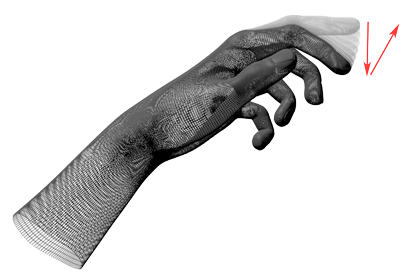
\includegraphics[width=0.5\textwidth]{images/keytap1}
            \label{kt1}
        }
        
        \quad
        
        \subfigure[Gesto con la mano también admitido.] {
            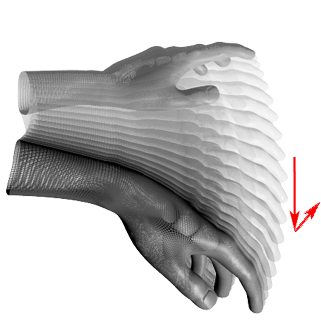
\includegraphics[width=0.5\textwidth]{images/keytap2}
            \label{kt2}
        }
    }
    
    \caption{Gestos para pausar la música.}
    \label{kt}
\end{figure}

\subsection{\textcolor{verde}Reproducir}

Este evento se activa cuando la canción que se estaba reproduciendo \textit{\textcolor{está pausada}}. Para poder volver a reproducir la canción, tenemos que hacer el mismo gesto que para pausar una canción. Estos gestos los podemos ver en la \hyperref[kt]{Figura \ref*{kt}}.

Cuando se lance este evento, el icono de pausa de la parte inferior izquierda de la pantalla cambiará al icono de reproducción. 

\subsection{\textcolor{verde}Pasar a la siguiente canción o a la anterior.}

Estos gestos son bastante similares entre sí, ya que ambos utilizan el gesto predefinido ``\textbf{\textit{\textcolor{verde}{swipe}}}''. Este gesto consiste en pasar la mano desde un lado hacia el lado opuesto pasando por encima del \textit{\textcolor{Leap}}.

Dependiendo del sentido en el pasemos la mano, podremos pasar o retroceder de canción:

\begin{enumerate}[$\bullet$]
  \item \textbf{\textcolor{verde}{De derecha a izquierda}}: 
  \item \textbf{\textcolor{verde}{De izquierda a derecha}}:
\end{enumerate}
\end{document}

